\documentclass{article}

\usepackage[english]{babel}
\usepackage[a4paper,top=2cm,bottom=2cm,left=3cm,right=3cm,marginparwidth=1.75cm]{geometry}
\usepackage{float}

% Useful packages
\usepackage{amsmath}
\usepackage{graphicx}
\usepackage[colorlinks=true, allcolors=blue]{hyperref}

\title{Callista Twilightshade}
\author{Karcag Tamas}

\begin{document}
\maketitle

\begin{abstract}
    Your abstract.
\end{abstract}

\section{Appearance of Callista}

\begin{figure}[H]
    \centering
    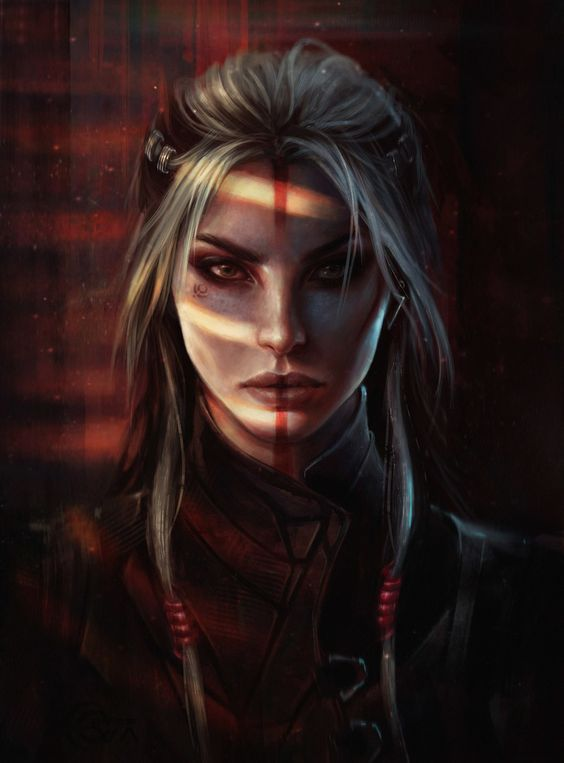
\includegraphics[width=0.6\textwidth]{Callista.jpg}
    \caption{\label{fig:callista}Callista portrait.}
\end{figure}

\textbf{Callista} is a mesmerizing \textbf{human woman} who possesses an ethereal beauty. Her \textbf{porcelain skin}, as fair as moonlight, carries a subtle hue of gray that lends an otherworldly charm to her appearance. Cascading down her back, her lustrous locks are a mesmerizing blend of white and gray, shimmering like strands of stardust. Framing her face, they accentuate her youthful features and add a touch of wisdom to her countenance.

Enchanting \textbf{yellow eyes}, reminiscent of a flickering flame, peer out from beneath elegantly arched eyebrows. They possess a captivating intensity, seeming to hold secrets and mysteries untold.

Her face, pale and flawless, is like a canvas waiting to be admired. Adorning it, a bold vertical line of \textbf{vibrant red paint} stretches from her \textbf{forehead} down to the tip of her nose, symbolizing a connection to ancient traditions and mystical rituals. This crimson mark, meticulously applied, accentuates her features, and highlights her innate allure.

Draped upon her lithe figure, \textbf{Callista} dons attire that echoes her enigmatic nature. Clad in supple \textbf{red leather garments}, they fit her form snugly, emphasizing her graceful curves and accentuating her feminine power. Intricate \textbf{purple borders} and mystical markings embellish her clothing, interweaving seamlessly with the scarlet fabric.

\begin{figure}[H]
    \centering
    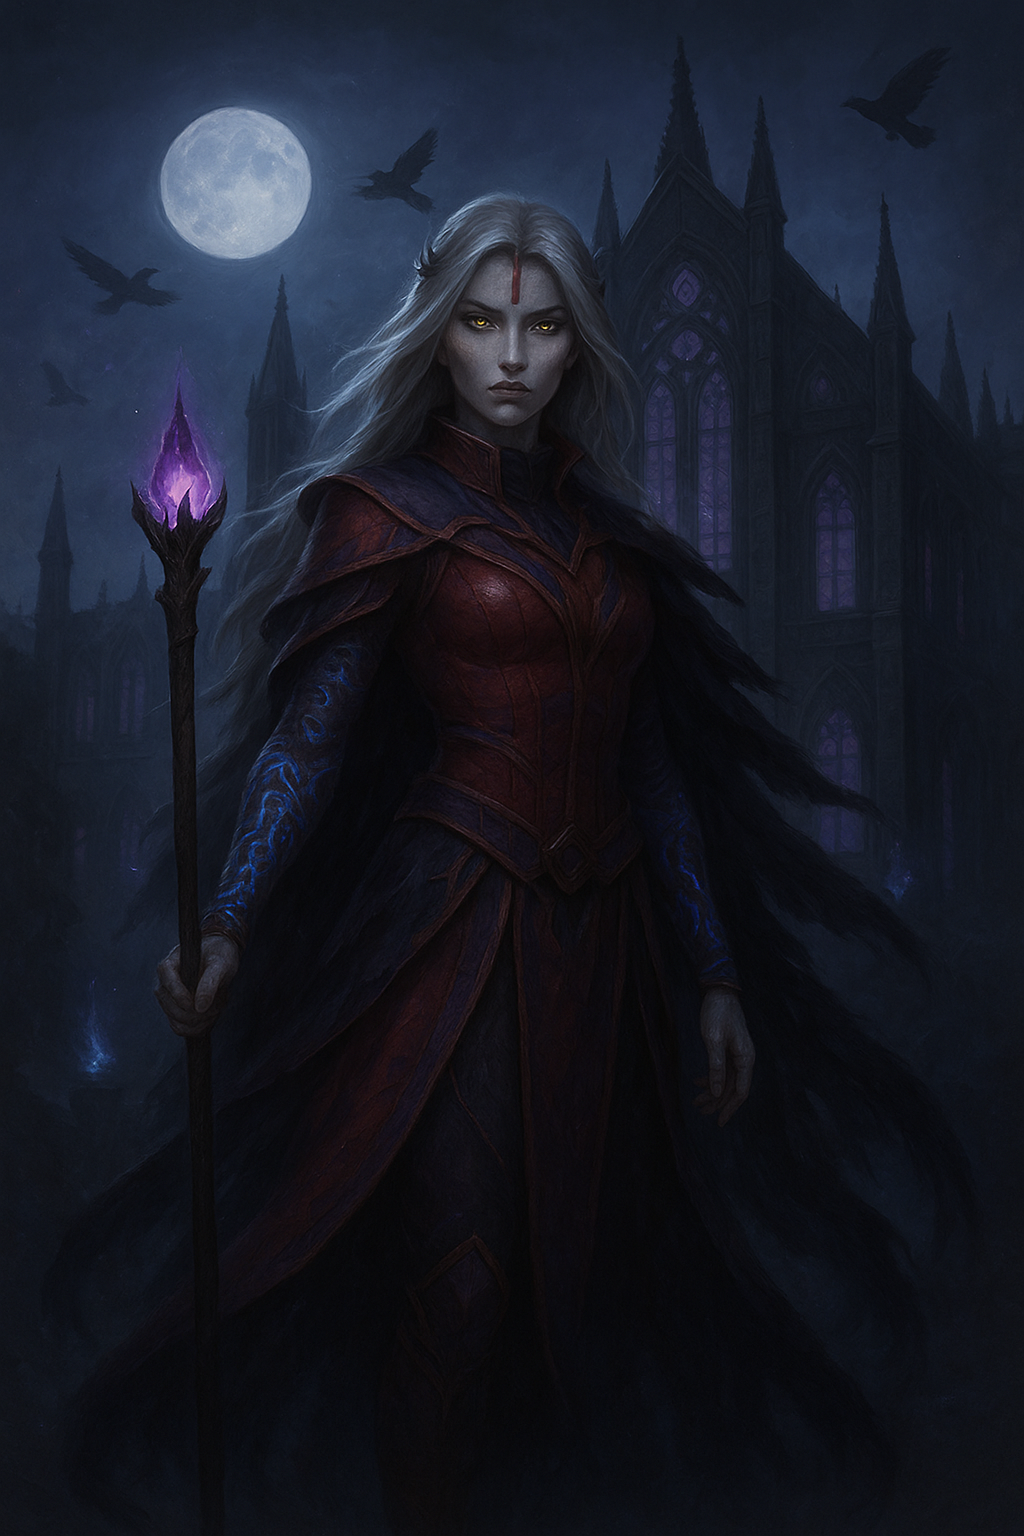
\includegraphics[width=0.6\textwidth]{Callista2.png}
    \caption{\label{fig:callista2}Callista.}
\end{figure}

Though she has gracefully aged to \textbf{57 years}, \textbf{Callista} possesses an everlasting youthfulness that belies her true age. She exudes the vibrancy and vitality of a woman in her early twenties, her ageless beauty captivating those who gaze upon her. Standing at a medium height of \textbf{165 centimeters}, she commands attention with her confident stance and regal bearing. Her lithe frame, toned and agile, reflects the dedication and discipline she possesses in her pursuit of arcane knowledge and physical prowess.

One of Callista's most intriguing traits is her \textbf{cold vision}. It grants her the ability to see the unseen, perceiving the invisible threads of magic that weave through the world around her.

\section{Behavior of Callista}

\textbf{Callista}'s demeanor reflects the \textbf{deep-seated emotions} within her, as she carries an \textbf{air of coldness} that seems to emanate from her very being. Her \textbf{icy exterior} acts as a shield, protecting her \textbf{vulnerable heart} from the harshness of the world.\ \textbf{Rarely} does a \textbf{smile} grace her lips.

Snarled and guarded, \textbf{Callista} \textbf{maintains a distance} from others, her walls fortified by the weight of her past experiences. It is not that she harbors ill intentions, but rather she struggles to find the trust and connection that she yearns for. Her \textbf{interactions with people are limited} and often strained, as she struggles to bridge the gap between her own isolation and the desire to fight for the world and its inhabitants.

Despite her solitary nature, \textbf{Callista} is driven by a \textbf{profound sense of duty} and a fierce determination \textbf{to protect the world} and its people. Her battles are not just physical, but also internal, as she grapples with the weight of her responsibilities and the sacrifices required in her pursuit of justice. The flame of her purpose burns bright within her, fueling her resolve to overcome the hardships that come her way.

When she does speak, her words carry a weight and intensity that demand attention.\ \textbf{Each syllable} is \textbf{chosen carefully, bearing the weight} of her convictions and the wisdom gained from a lifetime of hardships. Though her communication may be sparse, her words hold depth, resonating with those who take the time to listen.

Her commitment to the greater good drives her forward, pushing her to the brink of her capabilities. However, in the midst of the chaos and the battles, she often finds solace in the knowledge that her actions hold the potential to bring about positive change, even if it means bearing the \textbf{burden of loneliness and isolation}.

She is not only a guardian of life and memory but also a devoted vegetarian. Her commitment to a vegetarian lifestyle is a reflection of her reverence for all living beings, aligning with her belief in the sanctity of life. In a world where power often dictates actions, her choice to abstain from consuming animal products is a testament to her compassion and dedication to preserving the balance of life in all its forms.

\section{Background Story of Callista}

In the realm of \textbf{Celestia}, where the heavens and the mortal world intertwine, \textbf{Callista}, an \textbf{Aasimar sorceress}, was born. From the moment of her celestial birth, her path was intertwined with destiny, guided by forces beyond mortal comprehension.

\begin{figure}[H]
    \centering
    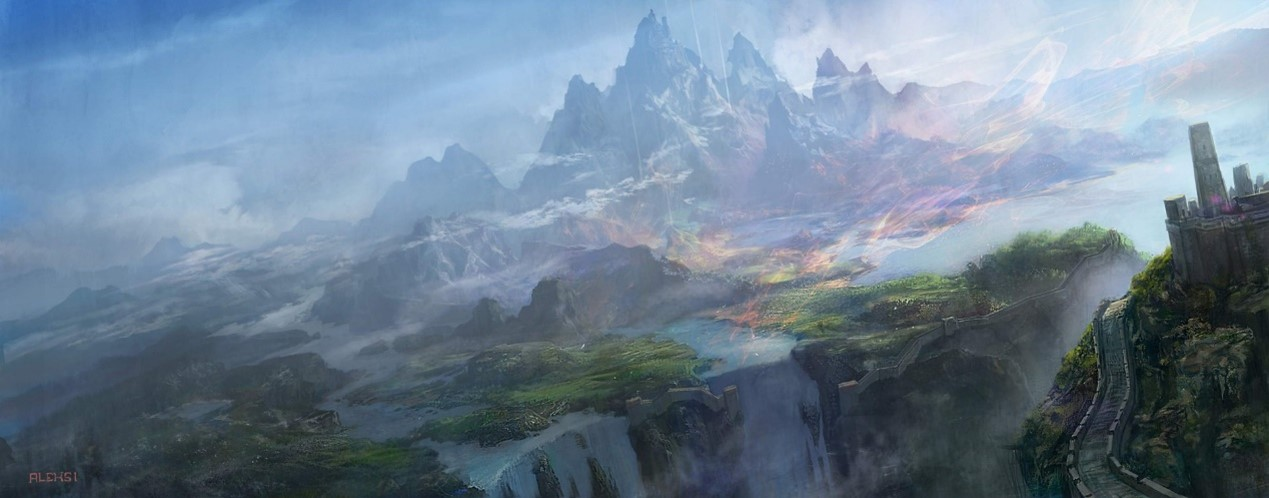
\includegraphics[width=1\textwidth]{src/Celestia.jpg}
    \caption{\label{fig:celestia}The Realm of Celestia.}
\end{figure}

Raised within a society that revered and celebrated the benevolent beings of the celestial realms, \textbf{Callista}'s existence was imbued with a sense of purpose and divinity. Her luminous presence, inherited from her celestial lineage, shone with an ethereal glow, captivating all who beheld her.

\subsection{Young Age}

During her early years, she was a remarkably \textbf{spirited} and \textbf{playful} young girl, until a profoundly sorrowful incident altered the course of her life. \textbf{Callista} had an older brother \textbf{(Dariel)} who held a deep affection for his younger sibling.

\begin{figure}[H]
    \centering
    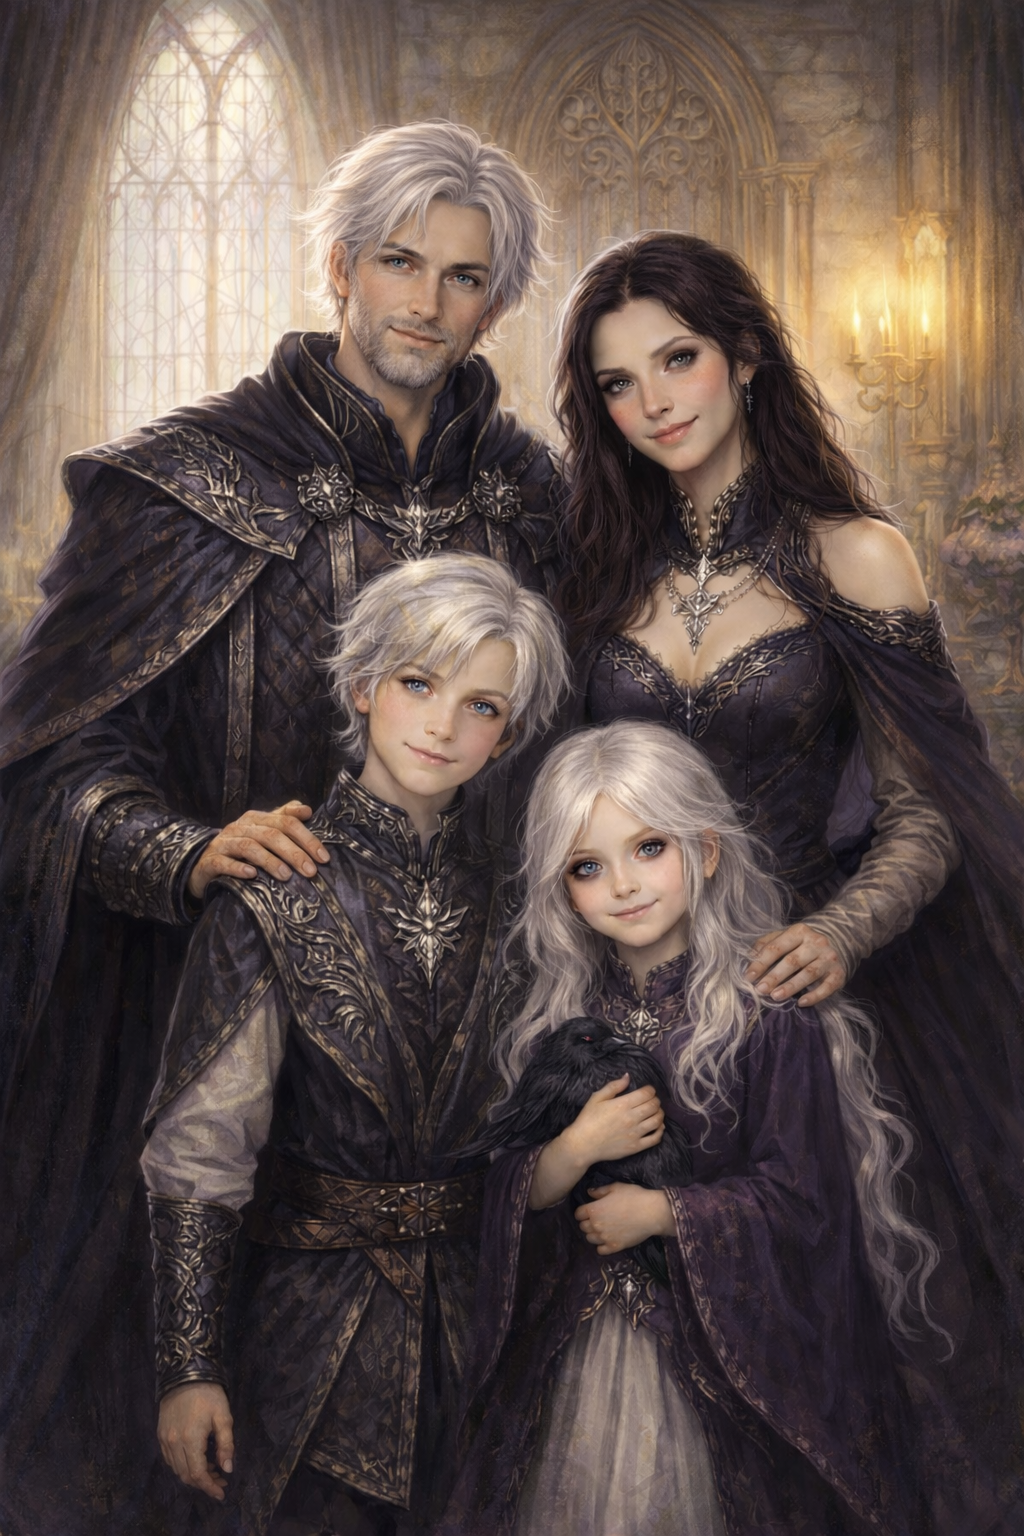
\includegraphics[width=0.6\textwidth]{src/Family.png}
    \caption{\label{fig:family}The Twillightshade family.}
\end{figure}

One fateful day, they ventured into the forest together, but their journey took a tragic turn when they fell prey to a gang of ruthless thieves. In a selfless act to shield \textbf{Callista} from harm, her brother valiantly engaged the bandits in combat. Although she managed to escape, her beloved brother never returned. Their parents, consumed by grief, perpetually held her responsible for the tragedy that befell their family.

Following that tragic event, \textbf{Callista} parted ways with her parents and resolved to embark on a quest to locate her brother. Although uncertain about his fate, she was inexplicably drawn to the lingering presence of her sibling. Despite years of relentless, yet fruitless searching, she eventually came to the realization that she needed to explore alternative avenues in her pursuit.

\subsection{Shadowfell}

However, as \textbf{Callista} matured, a growing fascination with the mysteries of the \textbf{Shadowfell}, a plane of darkness and shadow, began to take hold of her curious mind. Drawn to the enigmatic allure of this shadowy realm, she embarked on a journey of self-discovery, seeking to uncover the secrets that lay hidden within. She held the belief that the answers would be there.

During her travels, \textbf{Callista} stumbled upon a forgotten tome, its pages filled with ancient prophecies and esoteric knowledge. Within its weathered bindings, she found mention of the \textbf{Raven Queen}, a mysterious deity whose influence stretched across the planes, particularly in the realm of death. Intrigued by the tales of a goddess who commanded the powers of fate and memories, \textbf{Callista} became consumed by a desire to understand this enigmatic figure.

Driven by an insatiable thirst for knowledge, \textbf{Callista} embarked on a pilgrimage to the desolate \textbf{Shadowfell}, where the Fortress of Memories, the \textbf{Raven Queen}'s citadel, stood as a testament to her dominion over the souls of the departed. Guided by visions and the celestial whispers that echoed within her mind, \textbf{Callista} traversed the treacherous paths of the \textbf{Shadowfell}, braving the dangers that awaited her.

\begin{figure}[H]
    \centering
    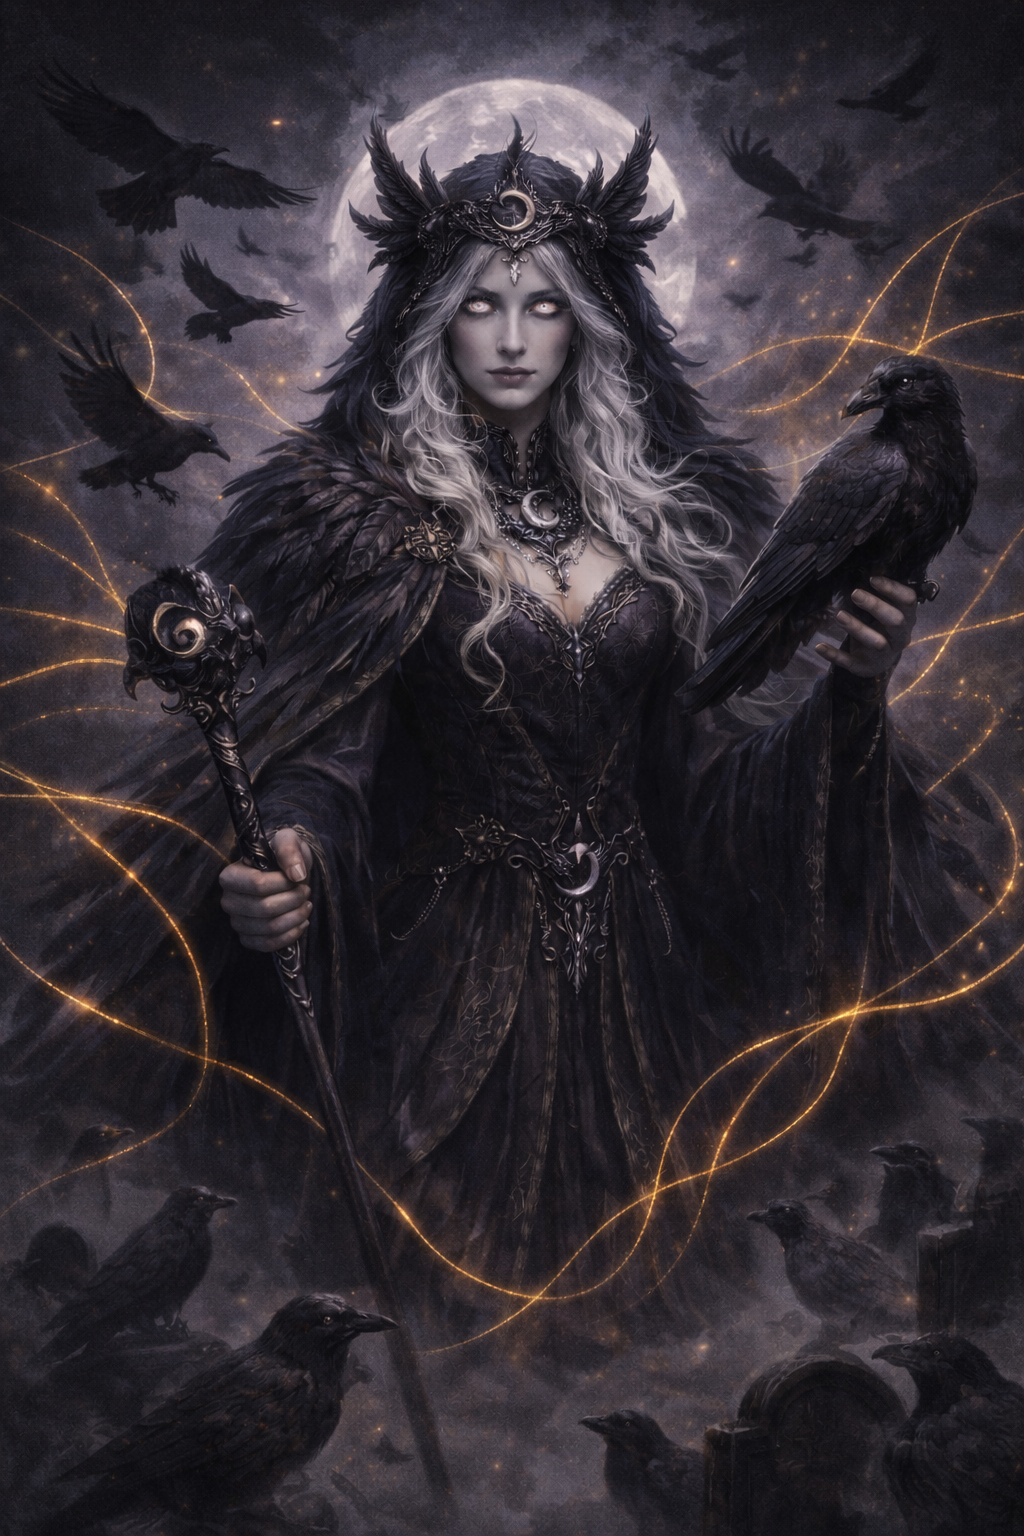
\includegraphics[width=0.6\textwidth]{src/RavenQueen.png}
    \caption{\label{fig:ravenqueen}The Raven Queen.}
\end{figure}

Upon reaching the towering gates of the Fortress of Memories, \textbf{Callista}'s conviction and unwavering faith in her quest granted her an audience with the \textbf{Raven Queen} herself. In that profound encounter, the deity recognized the unyielding determination and the thirst for understanding that burned within \textbf{Callista}'s soul. Impressed by the Aasimar's fervor, the \textbf{Raven Queen} offered her a pact—an opportunity to become her devoted follower and channel the powers of life, death, and the manipulation of memories. This presented a significant opportunity to reunite with her brother after a prolonged separation.

Accepting the \textbf{Raven Queen}'s offer without hesitation, \textbf{Callista} became forever bound to the divine will of her newfound patron. She relinquished a portion of her own mortality, forging a connection that allowed her to wield the mysteries of the \textbf{Shadowfell} and the ethereal powers of the celestial realm in tandem.

\begin{figure}[H]
    \centering
    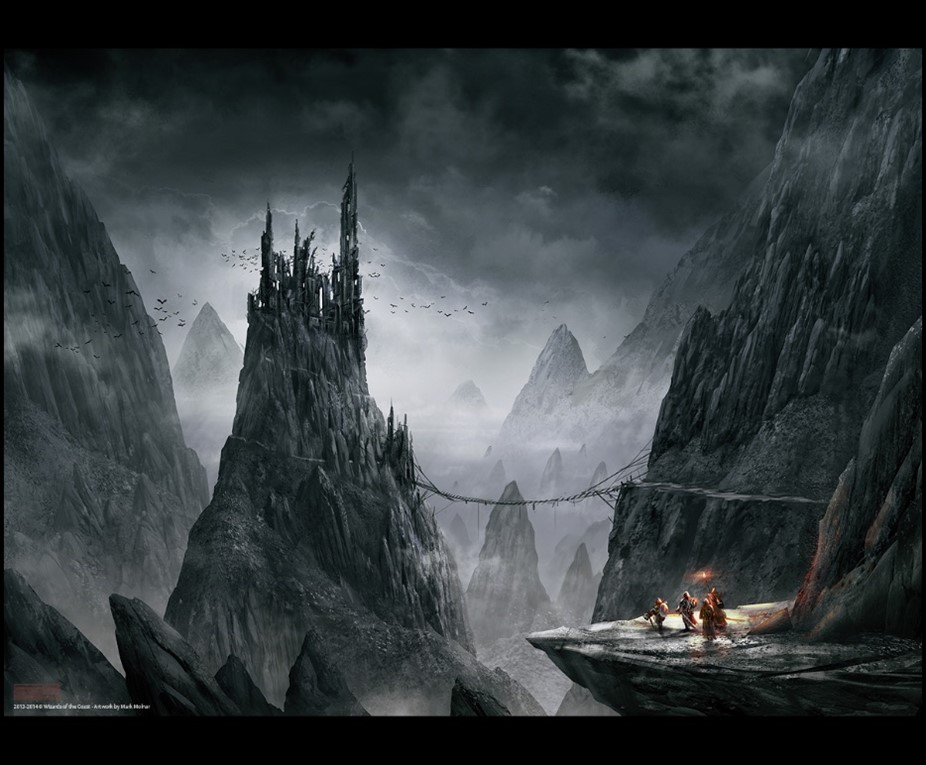
\includegraphics[width=1\textwidth]{src/Shadowfell.jpg}
    \caption{\label{fig:shadowfell}The Realm of Shadowfell.}
\end{figure}

\subsection{Love}

Despite the incredible potential this newfound power held, \textbf{Callista} found herself unable to employ it in her quest to locate her long-lost brother and rebuild the trust and affection of her family. Instead, she embarked on a series of adventures, seeking to understand her evolving self. Along her journey, she encountered a myriad of individuals, but unfortunately, many proved untrustworthy, unintelligent, or simply eccentric. She had little desire to delve deeper into their lives and swiftly distanced herself from them whenever possible.

In her battles, she confronted malevolent infernal entities, sinister abyssal monstrosities, and even common thugs in dimly lit taverns. Through these encounters, she came to understand the vulnerability of human minds, easily susceptible to manipulation by dark forces.

However, on a fateful day, \textbf{Callista} crossed paths with a woman named \textbf{Lysandra}, whose beauty was matched only by her kindness and inner strength. \textbf{Lysandra}, a young woman in her early twenties, possessed fiery red hair that perfectly matched her bold and unflinching gaze.

Their initial meeting lacked romance or emotional resonance. \textbf{Callista} embarked on a solitary quest in search of an ancient tome on necromantic magic, while \textbf{Lysandra}, suspicious of \textbf{Callista}'s intentions with the book, confronted her. Their clash escalated into a prolonged duel until they found themselves beset by formidable mountain cave-dwelling spiders. In that dire moment, they both realized that their survival hinged on cooperation.

Following a near-death battle, they forged a truce, extending a helping hand to nurse each other back to health. As they sat beside the campfire, their casual conversation gradually evolved into something profound and intimate, delving into depths neither had anticipated. In a singular moment, they experienced a soulful connection that set them apart from all others. Actions spoke louder than words, and that night, they shared an intimate unity, drawn together by an unspoken bond.

That fateful night became a turning point in their lives, an encounter marked by something extraordinary, something beautiful. However, at the outset, \textbf{Lysandra} sensed an unfamiliar emotion, perhaps fear – the fear of love, the fear of loss. When \textbf{Callista} awoke the following morning, \textbf{Lysandra} had mysteriously disappeared, leaving her with a profound sense of loneliness. The words of greeting remained unsaid, lost in the silence. Since that moment, \textbf{Callista} struggled to put \textbf{Lysandra} and the complex emotions she had stirred within her out of her mind. She attempted to deny these feelings, but deep within her heart, a glimmer of hope lingered, yearning for the possibility of seeing \textbf{Lysandra} once more.

\subsection{Adventures}

Now, \textbf{Callista}'s journey continues as a servant of the \textbf{Raven Queen}, traversing the realms and unraveling the secrets of life, death, and the intricate tapestry of memories. With each step, she delves deeper into her sorcerous abilities, tapping into the essence of her celestial heritage while embracing the enigmatic darkness that shrouds her path. As she carries out her duties in service to her divine patron, \textbf{Callista} treads the fine line between life and death, weaving her own fate and leaving an indelible mark on the tapestry of existence.

After years of dedicated service as a faithful servant of the \textbf{Raven Queen} and an accomplished adventurer within the empire, a remarkable opportunity unfolded before her. The emperor personally selected her to join a team of renowned adventurers, a group whose reputation had reached her ears long before. They were known for safeguarding the welfare of the people and upholding justice, with Rodrik Blackwood at the forefront of their noble efforts. They extended their aid to the vulnerable and oppressed. For \textbf{Callista}, this mission presented a glimmer of hope in her quest to find her long-lost brother, if indeed he still walked
among the living.

Will she reunite with her brother, or will fate once again cross her path with the enigmatic woman? Only time will unveil the answer to this lingering question.

\section{Dariel}

\begin{figure}[H]
    \centering
    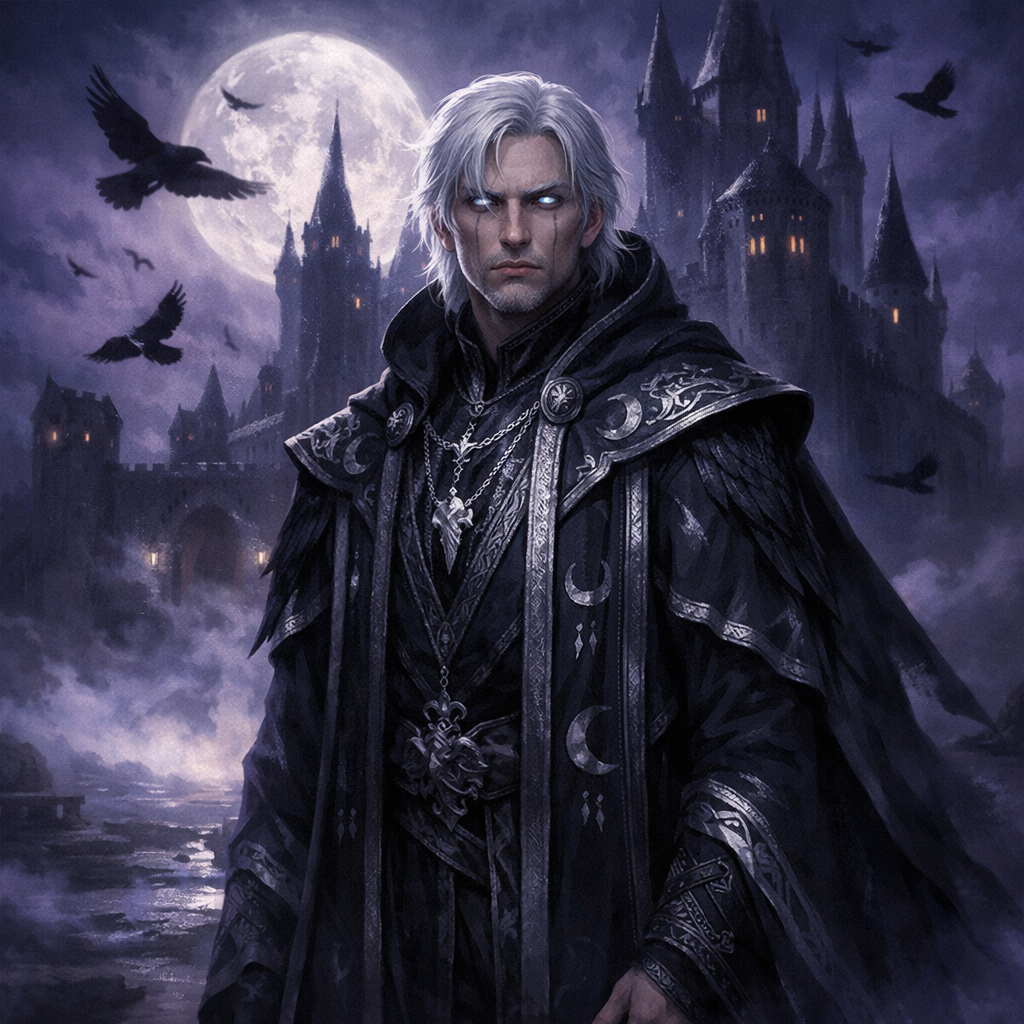
\includegraphics[width=0.6\textwidth]{src/Dariel2.png}
    \caption{\label{fig:dariel}Dariel.}
\end{figure}

\textbf{Dariel}, the eldest child and the older sibling of \textbf{Callista}, held a special place in their parents' hearts as the favored one, often regarded as the family's prodigious talent. He consistently outshone the rest. To \textbf{Callista}, he was not just a brother, but a cherished figure who constantly offered support and protection, someone she deeply admired.

In the wake of the heart-wrenching disappearance, \textbf{Callista} found herself consumed by despair. The uncertainty of her brother's fate weighed heavily on her, the question of whether he was alive or not haunting her every thought. But unbeknownst to her, her brother did survive. The bandits, instead of taking his life, opted to sell him for a sum of coin to a cult with a sinister agenda. They subjected him to a process of brainwashing, molding him into a lethal instrument of their evil plans. He became a pawn in their sinister machinations, a mere tool at their disposal.

Will their paths converge once more? Can her brother recognize his long-lost sister? Is there a chance to reunite the siblings? These questions hang in the balance, awaiting the answers that their forthcoming adventures will provide.

\section{Lysandra}

\begin{figure}[H]
    \centering
    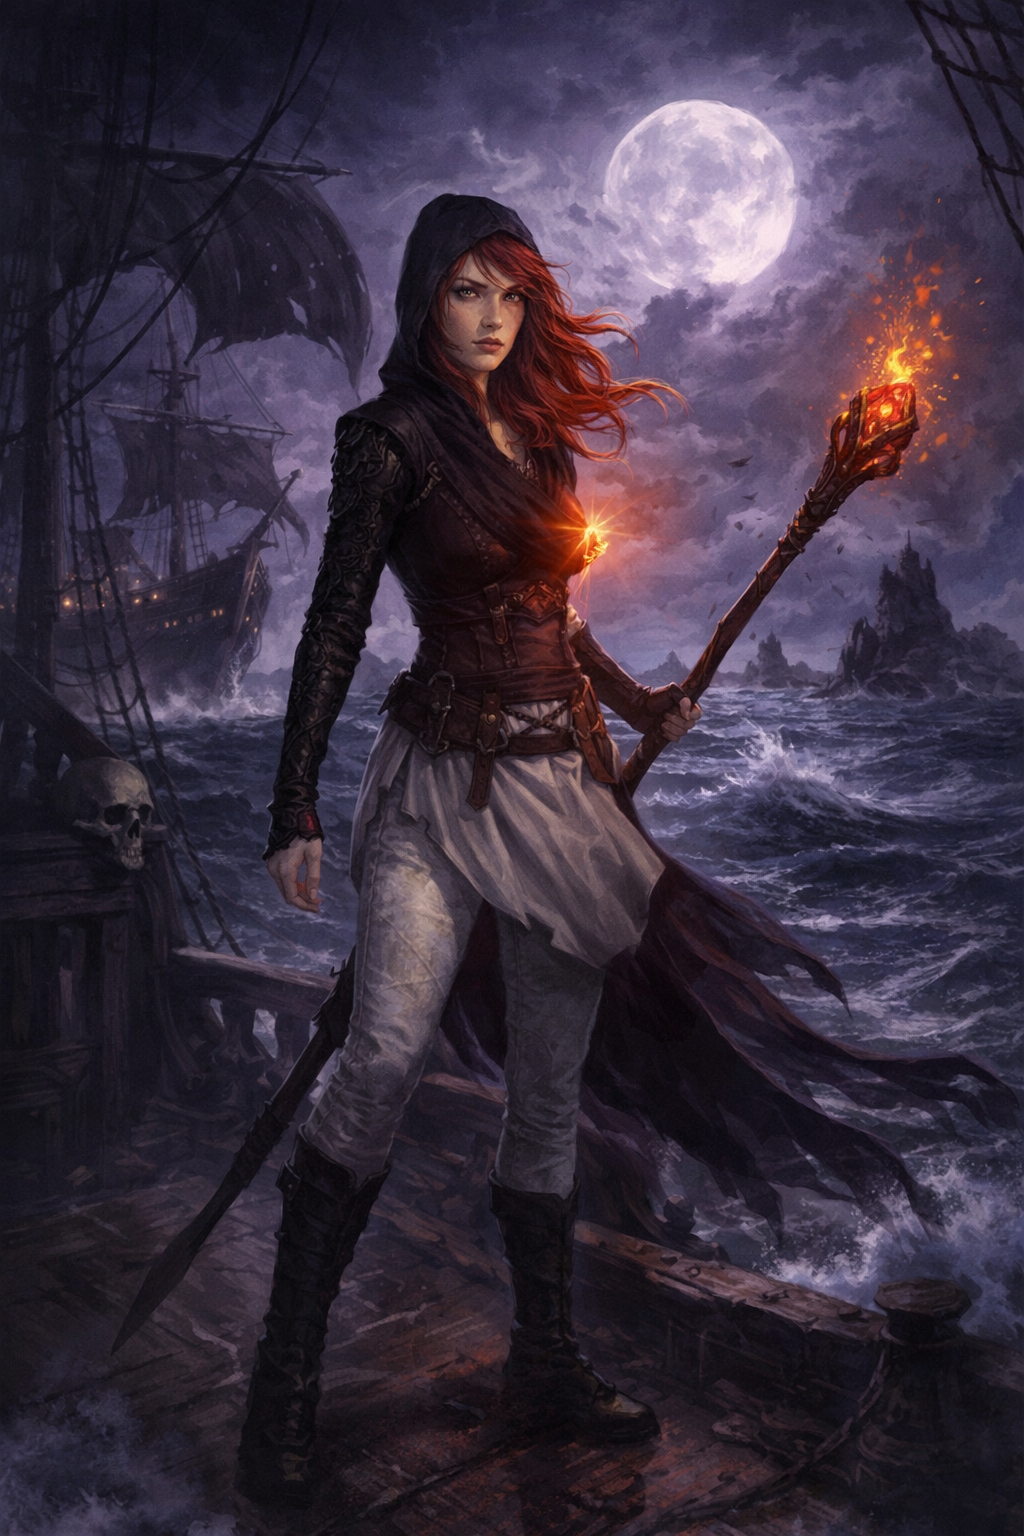
\includegraphics[width=0.6\textwidth]{src/Lysandra2.png}
    \caption{\label{fig:lysandra}Lysandra.}
\end{figure}

\textbf{Lysandra}, too, began her life as a cheerful and contented young girl. Growing up in a joyful human household alongside three elder brothers and a younger sister, her early years were filled with happiness. However, her destiny took a turn one fateful day at a carnival when she witnessed a magician whose performance left an indelible mark on her. Inspired by the magician's ability to bring wonder and joy, \textbf{Lysandra} resolved to use magic to aid others. Despite having no inherent magical lineage, she embarked on a journey to master the art of magic through dedicated learning and practice.

Following years of rigorous schooling, she embarked on a journey to master her magical talents. Among the various schools of magic, she found her true passion in the fiery arts, drawn to its vibrant and lively essence. To her, fire embodied life and happiness, a source of unyielding fascination. Her adventures led her down numerous paths, but it was on one particular day that her destiny intertwined with \textbf{Callista}'s. Upon meeting her, \textbf{Lysandra} detected an intriguing quality, something unique and extraordinary, a sensation entirely novel and unfamiliar to her.

This newfound emotion filled her with unease. Having never experienced a deep romantic connection before, she made the choice to distance herself from the situation. Yet, not a day passed without thoughts of \textbf{Callista} crossing her mind. She held onto the hope of encountering \textbf{Callista} once more, even as she grappled with the fear of that very prospect.

Will their paths cross once more? What will the circumstances of their reunion be like, marked by joy or awkwardness? And most importantly, will both find happiness in this meeting?

\end{document}